\documentclass[a4paper,12pt]{article}
\usepackage{caption}
\usepackage{float}
\usepackage{graphicx}
\usepackage{listings}
\usepackage{amsfonts}
\usepackage{amsmath}

\usepackage[utf8]{inputenc}
\usepackage{biblatex}

% Copyright 2017 Sergei Tikhomirov, MIT License
% https://github.com/s-tikhomirov/solidity-latex-highlighting/

\usepackage{listings, xcolor}

\definecolor{verylightgray}{rgb}{.97,.97,.97}

\lstdefinelanguage{Solidity}{
	keywords=[1]{anonymous, assembly, assert, balance, break, call, callcode, case, catch, class, constant, continue, constructor, contract, debugger, default, delegatecall, delete, do, else, emit, event, experimental, export, external, false, finally, for, function, gas, if, implements, import, in, indexed, instanceof, interface, internal, is, length, library, log0, log1, log2, log3, log4, memory, modifier, new, payable, pragma, private, protected, public, pure, push, require, return, returns, revert, selfdestruct, send, solidity, storage, struct, suicide, super, switch, then, this, throw, transfer, true, try, typeof, using, value, view, while, with, addmod, ecrecover, keccak256, mulmod, ripemd160, sha256, sha3}, % generic keywords including crypto operations
	keywordstyle=[1]\color{blue}\bfseries,
	keywords=[2]{address, bool, byte, bytes, bytes1, bytes2, bytes3, bytes4, bytes5, bytes6, bytes7, bytes8, bytes9, bytes10, bytes11, bytes12, bytes13, bytes14, bytes15, bytes16, bytes17, bytes18, bytes19, bytes20, bytes21, bytes22, bytes23, bytes24, bytes25, bytes26, bytes27, bytes28, bytes29, bytes30, bytes31, bytes32, enum, int, int8, int16, int24, int32, int40, int48, int56, int64, int72, int80, int88, int96, int104, int112, int120, int128, int136, int144, int152, int160, int168, int176, int184, int192, int200, int208, int216, int224, int232, int240, int248, int256, mapping, string, uint, uint8, uint16, uint24, uint32, uint40, uint48, uint56, uint64, uint72, uint80, uint88, uint96, uint104, uint112, uint120, uint128, uint136, uint144, uint152, uint160, uint168, uint176, uint184, uint192, uint200, uint208, uint216, uint224, uint232, uint240, uint248, uint256, var, void, ether, finney, szabo, wei, days, hours, minutes, seconds, weeks, years},	% types; money and time units
	keywordstyle=[2]\color{teal}\bfseries,
	keywords=[3]{block, blockhash, coinbase, difficulty, gaslimit, number, timestamp, msg, data, gas, sender, sig, value, now, tx, gasprice, origin},	% environment variables
	keywordstyle=[3]\color{violet}\bfseries,
	identifierstyle=\color{black},
	sensitive=false,
	comment=[l]{//},
	morecomment=[s]{/*}{*/},
	commentstyle=\color{gray}\ttfamily,
	stringstyle=\color{red}\ttfamily,
	morestring=[b]',
	morestring=[b]"
}

\lstset{
	language=Solidity,
	backgroundcolor=\color{verylightgray},
	extendedchars=true,
	basicstyle=\footnotesize\ttfamily,
	showstringspaces=false,
	showspaces=false,
	numbers=left,
	numberstyle=\footnotesize,
	numbersep=9pt,
	tabsize=2,
	breaklines=true,
	showtabs=false,
	captionpos=b
}
\usepackage{listings, xcolor}

\definecolor{verylightgray}{rgb}{.97,.97,.97}

\lstdefinelanguage{Vyper}{
	keywords=[1]{assert, keccak, keccak256, def, struct}, % generic keywords including crypto operations
	keywordstyle=[1]\color{blue}\bfseries,
	keywords=[2]{address, bool, byte, bytes, bytes1, bytes2, bytes3, bytes4, bytes5, bytes6, bytes7, bytes8, bytes9, bytes10, bytes11, bytes12, bytes13, bytes14, bytes15, bytes16, bytes17, bytes18, bytes19, bytes20, bytes21, bytes22, bytes23, bytes24, bytes25, bytes26, bytes27, bytes28, bytes29, bytes30, bytes31, bytes32, enum, int, int8, int16, int24, int32, int40, int48, int56, int64, int72, int80, int88, int96, int104, int112, int120, int128, int136, int144, int152, int160, int168, int176, int184, int192, int200, int208, int216, int224, int232, int240, int248, int256, mapping, string, uint, uint8, uint16, uint24, uint32, uint40, uint48, uint56, uint64, uint72, uint80, uint88, uint96, uint104, uint112, uint120, uint128, uint136, uint144, uint152, uint160, uint168, uint176, uint184, uint192, uint200, uint208, uint216, uint224, uint232, uint240, uint248, uint256, var, void, ether, finney, szabo, wei, days, hours, minutes, seconds, weeks, years},	% types; money and time units
	keywordstyle=[2]\color{teal}\bfseries,
	keywords=[3]{block, blockhash, coinbase, difficulty, gaslimit, number, timestamp, msg, data, gas, sender, sig, value, now, tx, gasprice, origin},	% environment variables
	keywordstyle=[3]\color{violet}\bfseries,
	identifierstyle=\color{black},
	sensitive=false,
	comment=[l]{\#},
	morecomment=[s]{/*}{*/},
	commentstyle=\color{gray}\ttfamily,
	stringstyle=\color{red}\ttfamily,
	morestring=[b]',
	morestring=[b]"
}

\lstset{
	language=Vyper,
	backgroundcolor=\color{verylightgray},
	extendedchars=true,
	basicstyle=\footnotesize\ttfamily,
	showstringspaces=false,
	showspaces=false,
	numbers=left,
	numberstyle=\footnotesize,
	numbersep=9pt,
	tabsize=2,
	breaklines=true,
	showtabs=false,
	captionpos=b
}

\addbibresource{bibliography.bib}

\title{Accountant pattern: Lightweight solution for embeded micropayments}
\author{Jaro Šatkevič, me@jaro.lt} 

\begin{document}

\maketitle

With rise of attempts to build decentralised platforms on internet with embeded
payment mechanisms into them, the need of high throughput micropayments solution
using crypto currencies is big as never before. Blockchain payments must be 
verified and stored by every node in the network, meaning that the node with the 
least resources limits the overall throughput of the system as a whole. Popular 
off-chain protocols, such as \textit{Lightning Network}, \textit{Raiden} or 
various \textit{Plasma} implementaitons, may provide solution micropayments using
cryptocurrencies, however they have own problems while using for high throughput 
micropayments in decentralised systems. 

In this paper is provided construction of embedable, lightweight micropayment 
protocol called \textit{"Accountant pattern"} which is essentially solution 
combining techniques of payment hubs and digital cheque based uni-directional 
channels. Such construct may be used in decentralised VPN, CDN or Video
streaming platforms and provides hundreds of thousands transactions per second
throughput while in same time is relatively easy to implement.

\newpage
\tableofcontents
\newpage

\section{Introduction}

Idea of building decentralised systems is not new but the main addition to the 
previous ideas about decentralised protocols is possibility to embed payment 
mechanisms into them.

In decentralised systems, there are quite a few situations when two parties that
don't have trust relationship between each other may want to perform mutual 
transactions. This is especially true in decentralised VPN network case.

Because all network participants can be anonymous there could be situations when
service \textit{consumer} will not be willing to pay up-front whole amount and 
service \textit{provider} will not be willing to deliver service without 
prepayment. In such situations service could be split into chunks provided in 
exchange for micropayments, so each party could potentially risk only tiny 
amount of funds. In such situation there may be a need of transacting between 
parties couple times a minute while sending tiny amounts (value of less than 1 
cent).

Thanks to cryptocurrencies now it's possible to embed decentralised payment
solution in trustless and permissionless way. Because of technical limitations 
some additional work have to be done however.

The backbone of cryptocurrencies is a technology called \textit{blockchain}. 
This technology requires each transaction to be stored on the ledger and 
replicate it over thousands of the network participants. This impose a 
fundamental limit of amount of transactions can be processed. Let's take two 
most popular blockchains Bitcoin and Ethereum. Their blockchains can provide
throughput of 3 to 25 transactions per second which causes high transaction 
fees and makes on-chain transactions too expensive for micropayments.

To overcome blockchain scalability problems several approaches have been 
proposed: 

\begin{itemize}
    \item \textit{\textbf{Speedup blockchain}} itself by changing some 
    fundamental components.
    \item Use \textit{\textbf{blockchain per project}} (sidechains, Cosmos and 
    Polkadot networks).
    \item \textit{\textbf{Plasma}} and other kinds of child-chain solutions.
    \item Payment and \textit{\textbf{state channels}} based solutions.
\end{itemize}

Most of proposed solutions are still in early stage of development and are not 
widely adopted. Each of them have their own pros and cons and there is no clear 
winner at the moment. This is one of reasons why most of modern decentralised 
protocols are still in early betas. Some have already working core solutions, 
however payments are usually the missing part. \\

\textbf{The goal} of this work is to research simplest possible but still cheap 
and powerfull solution for high throughput micro payments using utility tokens
and easy embedable into decentralised VPN, CDN or streaming services.\\

\textbf{Following tasks} have to be accomplished to fulfill the goal of this work:
\begin{enumerate}
    \item Analyse needs of decentralised VPN, CDN or streaming platform and 
    collect requirements for payment solution which could be used there;
    \item Do research of several most promissing 2nd layer solutions such as 
    state channels, micropayment channel Networks, Plasma and Sidechains. Look
    over possibility to use them as base for high throughput micropayments in 
    decentralised platforms, describe their advantages, limitations and side 
    effects.
    \item Provide lightweight, easily embedable solution for high throughput 
    micropayments.
\end{enumerate}

\section{Platfrom review and requirements for payment solution}

Let's take Mysterium -- decentralised VPN platform as example where proposed 
micropayments solution can be used.

Mysterium Network is a network of nodes providing security and privacy to 
Mysterium end users via dVPN application. Combining powerful encryption, 
reputation mechanisms and layered protection protocols team ambition is to build
an infinitely scalable P2P architecture. The main difference of dVPN comparing
to other VPN service providers in the market is their architecture with 
decentralisation at the core. There should be no sigle failing part in the 
network. Any government, company or person should not be able to censure or stop
this service. Mysterium team itself should be not able to censure or stop work
of network, after final solution will be released into production.

At the moment product itself is in beta testing and is missing scalable payments
solution to go into public.

\subsection{Components of the network}

\begin{itemize}
    \item \textbf{Provider nodes:} service written in golang which can be run by
    any user of network to provide their bandwidth for other users (called 
    consumers) using OpenVPN in exchange to earning MYST tokens.
    \item \textbf{Consumer app:} software written in golang and JavaScript which
    can be run by any user in the network to connect to \textit{provider nodes} 
    via OpenVPN and use their bandwidth.
    \item \textbf{Discovery service:} decentralised service which helps
    providers to advertise themself in network so consumers would find them and 
    use their bandwidth.
    \item \textbf{Myst token:} internal crypto currency used in the network and 
    main and the only method of peyments. Myst token is released as ERC20 token 
    on Ethereum blockchain.
    \item \textbf{Identity:} each user of the network (both, consumers and 
    providers) have to register own identity, which is similar to ethereum 
    address (20 bytes of keccak256 hash of public key derived from private key 
    using eliptic curve cryptography). It is needed to uniquely identify network
    actors and to be able securly establish encripted connection between them. 
    Identity have to be registered on-chain using smart-contract deployed into 
    Ethereum network.
\end{itemize}

\subsection{Initially proposed payment solution}

Initially Mysterium team was planning to use mechanism which remotely resembles 
the way cheques works. A blockchain account holder can write a cryptographic 
cheque to another account (the beneficiary) as a form of payment. A cheque has 
the issuer's address, beneficiary's address, sum of tokens promised, sequence 
and signatures. Amount written on the cheque can be updated and only the last 
version of cheque is valid. Later beneficiary can settle promissed amount on 
blockchain. 

Here is snippet from smart contract code which should settle promised value 
on-chain.

\begin{lstlisting}[language=Solidity]
    function settlePromise(address issuer, 
                           address beneficiary, 
                           uint256 seq, 
                           uint256 amount, 
                           bytes issuerSignature,
                           bytes beneficiarySignature) public {
        bytes32 promiseHash = keccak256(beneficiary, seq , amount);

        address recoveredIssuer = ecrecover(promiseHash, issuerSignature);
        require(recoveredIssuer == issuer);

        address recoveredBeneficiary = ecrecover(promiseHash, beneficiarySignature);
        require(recoveredBeneficiary == beneficiary);

        require(seq > clearedPromises[issuer][beneficiary]);
        clearedPromises[sender][receiver] = seq;

        require(token.balanceOf(issuer) >= amount);
        token.transferFrom(issuer, beneficiary, amount);

        emit PromiseSettled(issuer, beneficiary, seq, amount);
    }
\end{lstlisting}

This solution is much better than doing on-chain transactions. Cheques with 
promised amounts can be send from consumer to provider even each second and be
send in peer-to-peer manner. Only \textit{consumer} and \textit{provider} will
be aware of their existance and only once in a while \textit{provider} will have
to settle transactions into blockchain. This helps to reduce on-chain 
transactions amount a lot and still having quite secure way of providing service
for untrusted party which can disapear at any moment. 

\subsubsection{Problems of digital cheques}

There are couple of critical problems however, and they have to be fixed. First 
of all there may be situation when there are not enought funds on issuer's 
balance to cover promised value in the blockchain so settling transaction will 
be rejected. This creates \textit{double spending} possibility, when after 
issuing cheque and until cheque is settled into blockchain, consumer still can 
try issue cheque of same funds to another party or even himself. In case of VPN 
service this is not that big problem because bandwidth is \textit{"perishable 
product"} and service providers can afford having part of it unpaid. Howewer 
such risk of double spending possibility pushes to more often on-chain 
settlements (each time when promised amount is big enough so risk of loosing 
money is not acceptable anymore).

Second problem is that most of consumers will use providers services only once 
and only for limited time (e.g. one hour of listening music), so providers will 
get a lot of small value cheques (e.g. 0.10 EUR value in tokens). On Ethereum 
to settle one such cheque can cost from 0.01 till 1 EUR depending on network 
busyness. This means that either big fees will be paid or cheques will be never 
settled.

\subsection{Requirements for "ideal" payments solution}

Because of high level of privacy and anonymity in decentralised networks, actors
of the network may don’t trust each other and there is no trusted intermediary 
available which could resolve conflicts or act as custodian service. In such 
situations \textit{Consumer} will be not willing to pay up-front whole amount 
and service \textit{Provider} will be not willing deliver service without 
prepayment. In such situation service could be split into microservices and be 
provided in exchange for nanopayments, so each party could potentially risk only 
tiny amount of funds. 

This leads into using \textit{pay-as-you-go} payment model where consumers are 
paying constantly, right after receiving agreed part of service. There may be a 
need of transacting between parties couple times a minute while sending tiny 
amounts.

\begin{enumerate}
    \item \textbf{requirement: consumer to provider payments}\\
    Usually there are two actors in the network, \textit{Consumers} and 
    \textit{Providers} of the service. All payments are done by 
    \textit{Consumers} and received by \textit{Providers} and never vice versa.

    There may be more complicated services where there can be more than two 
    parties. E.g. Video streamer (person who is creating content), nodes which 
    are streaming video and video viewers. In this case we still can separate 
    all of them into \textit{Consumers} and \textit{Providers}, just some 
    actors (e.g. nodes in this case) will have both of these roles, depending 
    on situation. In each pair (\textit{streamer-node} and \textit{node-viewer}) 
    payments will be still done only in one direction.

    Thanks to this observation the protocol can be simplified and take use of 
    \textit{payment promises} or \textit{uni-directional} micropayment channels.

    \item \textbf{requirement: high throughput and scalability}\\
    It is extremely important that protocol would support frequent payments of
    tiny amount (e.g. each 10 seconds by all participating parties of value less
    than 1 cent). Which means that:
    \begin{itemize}
        \item payment solution should be able to process as many transactions 
        per second as there are active sessions established between service 
        providers and consumers;
        \item value of transaction can be set to parts of cent (in given crypto
        currency);
        \item transactions should be marked as final in very short period of 
        time (ideally should have \textit{instant finality} property);
        \item there have to be fast answer about transaction status with minimal
        networking errors and retries amount;
        \item transaction fee have to be very small (parts of penny) or 
        expressed as percent of transaction value;
        \item there should be minimal presence on-chain, it have to be possible
        to aggregate payments of many sessions and from different consumers and 
        settle them on-chain at once.
    \end{itemize}

    \item \textbf{requirement: utility tokens and stable coins support}\\
    Bitcoin, Ethers or other popular crypto currencies are volatile and may be 
    not acceptable or too risky in some cases. Also there are many decentralised
    apps who have issued their own utility tokens (\textit{MYST} token in case
    if Mysterium Network). This means that there is requirement for payment 
    protocol to support transactions using \textit{ERC20} tokens issued on 
    Ethereum blockchain.

    \item \textbf{requirement: secure}\\
    Digital services such as VPN could be named as \textit{"perishable"} because 
    they actually are selling trafic which if not used, is "gone" forever. This 
    means that some level of risk of unpaid use of service can be acceptable. 
    However it's should be decision of each service provider what level of risk, 
    in exchange to increased usability and performance or lower on-chain 
    settling fees, he can take. So in general case, double spending attempt have 
    to be imidiatelly identified and such transactions should be rejected.

    Anonymity and permissionless nature of decentralised systems creates some 
    cases where additional level of protection against bad acting service 
    providers and consumers is needed. For example in decentralised VPN case, 
    pure performing service providers may try to "clean" their raiting by simply 
    creating new identity in the system. Bad acting consumers may organize DDoS 
    attack and for providers it will be hard to ban them, because they may 
    continuously create new identities. To prevent such behaviour there could be 
    used either some kind of identity registration with staking and punishment 
    system.

    \begin{itemize}
        \item network identity have to be registered in given smart-contract, to
        do so there should be paid registration fee or staked given amount of 
        tokens;
        \item there should be not possible to pay with same coin twice (avoid 
        double spending);
        \item system should be secure against different kind of attacks (e.g. 
        DDos);
    \end{itemize}

    \item \textbf{requirement: decentralised}\\
    Such important component as payments should have high level of liveness. 
    There should be no central party which would be easy to shutdown or censor. 
    This means that needed payment protocol should maintain at least some level 
    of decentralisation and should be not operated by single party.

    \item \textbf{requirement: low implementation complexity}\\
    There are couple of potential ways of embeding payment solution into 
    decentralised platform. It have to be either already very popular and 
    scalable payment network which works on many platforms, has easy and stable
    APIs and is already used by many people in many other platforms. Or it have 
    to be solution with low level of complexity so it would be easy to implement, 
    cheap to operate and resource efficient to use it.

    \begin{enumerate}
        \item \textbf{Easy implementation.} Because such protocol can be used in 
        various solutions and be slightly modificated for needs of particular 
        system, it have to be possible reimplement all it's main parts in any 
        popular programming language in a matters of weeks. As little of 
        complicated schemes or components should be used.
        \item \textbf{Cheap to operate.} To make solution easier to decentralise 
        it should be relatively cheap run and operate its nodes. No big initial 
        finantial investment, complicated installation and advanced hardware 
        should be required.
        \item \textbf{Efficient usage.} Because there is requirement to make 
        stable and fast payment solution, less communication messages have to be
        send via network between parties, less intermediaries involved, better 
        for the protocol.
    \end{enumerate}

    \item \textbf{requirement: good user experience}\\
    Not only technical parameters are important for successful systems. If it 
    is hard for user to make payment, only minority of them will stay to use 
    services. There are various angles of usability which ideally should be 
    solved.

    \begin{enumerate}
        \item Consumers should be able to deposite funds using any popular 
        crypto wallet or directly from exchanges.
        \item Users should have possibility to own just one asset (e.g. MYST
        token) and not be required to own any additional utility token or coin 
        used to pay for payment network. This is especially important while 
        using tokens on Ethereum where for each transaction have to be paid 
        some amount of ethers.
        \item Any cryptographic proofs should be able to be transfered not only
        by signing party, but also by any third party. In the same time they 
        have maintain same level of security. This allows to use cloud trustless
        services to send, validate or protect transactions.
        \item Because service providers are earning income on the system, they 
        can be asked for some kind of stake or platform fee. Consumers however 
        have to be able to avoid such requirements.
    \end{enumerate}
\end{enumerate}

\section{Overview of potential solutions}

\textit{Blockchain} is a replicated state machine which orders transactions on 
it's global state. Transactions are verified and replayed by each participant,
called a \textit{node}, in the network. This limists the throughput of the 
network as a whole to the lowest throughput of any of it's nodes. Increasing 
the load beyond that throughput may result in nodes unable to handle the load 
being pushed out of the network. This impose a fundamental limit of amount of 
transactions which can be processed. 

Let's take two most popular cryptocurrencies Bitcoin and Ethereum. Their 
blockchains can provide throughput of 3 to 15 transactions per second which in 
busy period causes high transaction fees and makes on-chain transactions too 
expensive for micropayments.

One of solutions would be to increase block size which could allow increase 
throughput. There are blockchains with block limits of 128Mb (100 times higher 
that bitcoin's) so theoretically they can process up to couple of hundreds 
transactions per second. Such level of scalability work for one-time type of 
payments (like buying cup of coffee) but for high throughput nano payments we 
need solution which could process millions of transactions per second. 
Unfortunatelly there are phisical network, validation time (CPU) and disk space 
limits so blocks can't be ultimately big.

Finally there is one more problem. Participants in the network by default agree 
that the chain with the highest \textit{difficulty} or more blocks put into it, 
is “true ledger”. If some other branch mined in parallel will get longer chain, 
a new ledger is accepted as the true ledger. Some transactions accepted into 
older ledger can be not added into new one. This means that the longer waiting 
period before accepting payment, the bigger guarantee the transaction written 
in blockchain is irreversible.

For frequent transactions, the faster \textit{finality} there is, the better. 
\textit{On-chain} transactions however don't have reasonably fast finality.\\

To overcome \textit{on-chain} limitations, such as scalability, high fees and
long finality time, several \textit{off-chain} protocols (or so-called 
\textit{Layer 2} solutions) have been proposed. Among these techniques, one 
important differentiator is whether the relocated operations introduce 
additional consensus assumptions (like in sidechains and interoperable 
blockchain networks such as Polkadot or Cosmos), or allow users to restore their
state to the original blockchain (like in state channels or Plasma).

\subsection{Blockchain per project}

The most radical solution would be to move platform specific utility token into 
own blockchain. There are couple of frameworks to build own blockchains with 
plugable consensus and application layer. Most promissing solutions are 
\textit{Tendermint} developed by Cosmos Network, \textit{Substrate} developed
by Parity Technologies as part of Polkadot Network, using software of Ethereum
but with different consensus algorithm and \textit{Hyperledger Fabric} by Linux
Foundation.

Nevertheless that these solutions are relatively hard to customise and launch, 
using them would additionally require building community of full nodes and stake 
pools which would guaranty network's security. Another unwanted side effect 
would be need of moving token into new blockchain. This is socialy complicated 
and hard to implements project. \\

Alternatively there could be launched a \textit{sidechain} - a blockchain ledger 
that runs in parallel to a primary blockchain. Assets from the main blockchain 
can be linked to and from the sidechain. This allows the sidechain to operate 
independently of the primary blockchain by introducing own consensus mechanism, 
faster speed of transactions and features needed to some dedicated platform.

\begin{figure}[H]
    \centering
    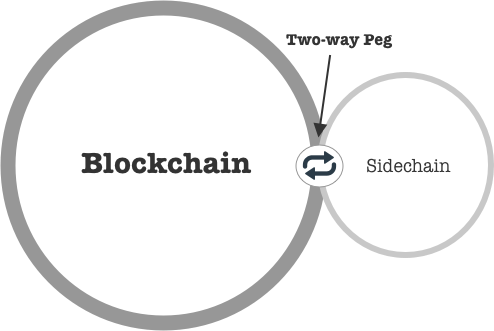
\includegraphics[scale=0.5]{img/sidechain}
    \caption{Two-way pegged sidechain}
    \label{img:sidechain}
\end{figure}

Thanks to possibility to use own, less decentralised but more scalable consensus
algorithms, \textit{sidechains} can provide much higher throughput than in 
primary blockchain. However while introducing consensus assumptions which in 
situation of fail will permanently compromise long-term guarantees (such as 
persistence of asset ownership). If state is "moved" to a sidechain and that 
chain's consensus mechanism fails, owners or beneficiaries of that state may 
lose everything delegated there, even when the primary blockchain remains
secure.

Slightly different approach is taken by interoperable multi-chain networks such 
as \textit{Polkadot} (see figure \ref{img:polkadot}) which allows new designs of
blockchains (called parachains) to communicate and pool their security while 
still allowing them to have the entirely arbitrary state-transition functions. 
This helps to bootstrap new chain much faster while having same security 
guaranties as whole Polkadot network.

\begin{figure}[H]
    \centering
    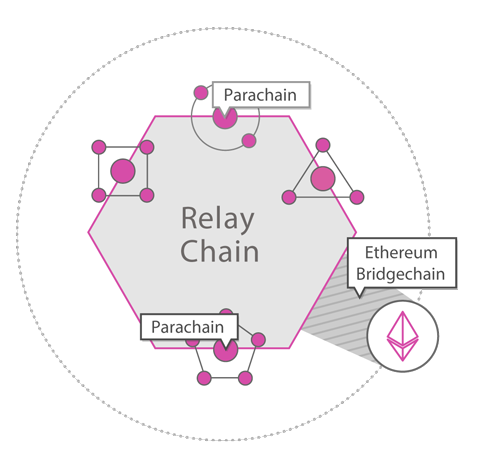
\includegraphics[scale=0.5]{img/polkadot}
    \caption{Polkadot network components}
    \label{img:polkadot}
\end{figure}

Despitethe the fact that \textit{sidechains} can provided significant increase 
of transaction throughput and in case of \textit{multi-chains} also relatively
easy achievable high level of security guarantees, general issues of blockchains
still apply. Because of blockchain nature and physical networking and storage 
limitations, they still can't provide throughput of hundreds of thousands 
transactions per second and \textit{instant finality}, which may be needed for 
\textit{micropayments} in succesfull decentralised VPN or streeming platform.

\subsection{Plasma}

\textit{Plasma} \cite{plasma} is a proposed framework for scaling Ethereum 
capacity by using hierarchical sidechains. Plasma type of sidechains (also 
called child chains) allow to do a majority of transactions outside of the "root
chain" (e.g. Ethereum). Only deposits and withdrawals, the points of entry and 
exit, are handled on the root chain smart contract.

Similary to blockchains Plasma chain stores all it's transactions packed into 
blocks while using \textit{UTXO} for balance accounting. To make sure that 
transactions are final, Plasma operator is doing something called a "state 
commitment". It is a cryptographic way to store a compressed version of the 
state of child-chain inside of root chain. Typically all the state is stored in
\textit{merkle trees} and only \textit{merkle root} of each block's state is 
persisted into root chain.

Usually Plasma chains are run by single operators, having distributed nodes 
using some kind of Byzantine Fault Tolerant (BFT) consensus (e.g. Proof of 
Stake) is possible though.

Differently to sidechains and multi-chains, Plasma makes possible for users to 
leave at any time. Such action is usually refered as “exiting”. This allows users 
safely withdrawal their funds out of Plasma even if it was shutdown by operator.

While it offers significant speed (up to 1000 tx/s) and latency improvements 
over Ethereum itself, Plasma cannot offer the near-zero latency and near-free 
transaction fees. It also requires significat storage to store it's ledger
(esoecially with big amounts of transactions).\\

Another downside of Plasma chais is that it is complex and difficult to 
implement solution. Especially hard is to run it with distributed nodes which 
have BFT type of consensus. When Plasma chain is operated with single operator, 
there is risk that he will create 'fake' blocks, which may end up with mass 
exits out of plasma into root chain and stuck of whole network.\\

One more downside is that plasma is quite expensive to operate. Each couple of 
blocks it have to commit it's state to root chain, which means, that plasma 
operator would have to pay 1080 USD (as gas fee) per day. 

\[ 3 \thinspace tx / minute * 1 440 \thinspace minutes / day = 4320 \thinspace tx/day \]
\[ 1 \thinspace tx = 25 \thinspace cents \]
\[ 4320 \thinspace tx/day * 0.25 USD/tx = 1080 \thinspace USD/day \]

This isn't big problem when there is already significant load in the network, 
however in the beginning covering such costs can be problematic.\\

And finaly, regardless of that Plasma transaction throughput is significantly 
higher than Ethereum's, it is still not enought for distributed VPN network 
needs. As alternative, there could be possible to build some kind of payments 
channels on top of Plasma (see \ref{img:plasma-channels}). In this way parties 
could do peer-to-peer transactions while having active service and close 
channels right after closing connection. 

\begin{figure}[H]
    \centering
    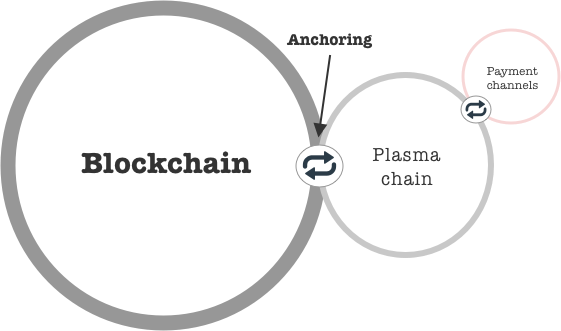
\includegraphics[scale=0.5]{img/plasma-channels}
    \caption{Plasma + payment channels}
    \label{img:plasma-channels}
\end{figure}

In situation when there are more that one transaction per second throughput, 
Plasma transactions can be relativelly cheap (less that 1 cent per transaction)
and can have fast including into block (from 1 to 10 seconds, depending on 
implementation). This allow opening and closing channels when needed and avoding
long waiting times.

Unfortunatelly this solution is even more complicated that using just plasma and
has similar cost and decentralisation issues mentioned above.

\subsection{Payment and state channels based solutions}

A \textit{micropayment channel} is class of techniques designed to allow parties
to exchange digital value without commiting all of the transactions to the 
blockchain. In a typical payment channel, only two transactions are added to the 
blockchain but an unlimited or nearly unlimted number of payments can be made 
between participants.

\begin{figure}[H]
    \centering
    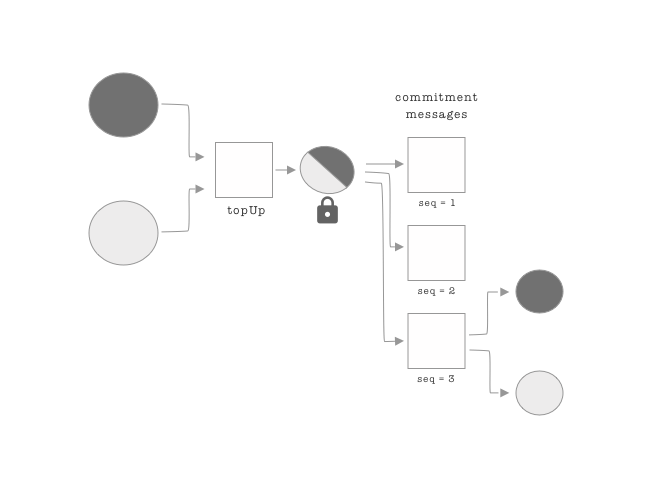
\includegraphics[scale=0.5]{img/payment-channel}
    \caption{Sequense based payment channel}
    \label{img:payment-channel}
\end{figure}

To open payment channel parties have to lock some funds into multisignature 
smart contract (see figure \ref{img:payment-channel}). This allows parties to
updated channels balances off-chains while beeing sure with hight probability 
that funds will be not double spent or stolen.

There are various payment channels techniques such as sequence based channels, 
duplex channels, time-locked channels, etc. Any of them would improve security 
and would help to avoid double spending problems comparing to initially proposed
digital cheques solution (see section 2.2). Also that would allow providers to
wait longer until settling on-chain what could reduce settling costs because 
some consumers may return to use service via same provider again. \\

\subsubsection{State channels}

State channels are the general form of \textit{payment channels}, applying the
same idea to any kind of state-altering operation normally performed on a 
blockchain. Moving these interactions off of the chain without requiring any 
additional trust can lead to significant improvements in cost and speed. State 
channels will be a critical part of scaling blockchain technologies to support 
higher levels of use.

The basic components of a state channel are very similar to that in payment 
channels.

\begin{enumerate}
    \item Part of the blockchain state is locked via multisignature type of smart 
    contract, so that a specific set of participants must completely agree with 
    each other to update it.
    \item Participants update the state among themselves by constructing and 
    signing transactions that could be submitted to the blockchain, but instead 
    are merely held onto for now. Each new update "trumps" previous updates.
    \item Finally, participants submit the state back to the blockchain, which 
    closes the state channel and unlocks the state again (usually in a different 
    configuration than it started with).
\end{enumerate}

Because tokens on Ethereum blockchain are represented in form of state in smart 
contracts, state channels are the way how to move token interacion into 
\textit{layer 2}.\\

\subsubsection{Downsides and benefits of channels}

The downside of using payment channels is that parties have to lock funds into 
multisigature smart contracts which in comparison to \textit{digical cheques} 
means additional on-chain transaction for opening channel and needs of having 
locked bigger amounts of funds. There is not possible to reuse same funds in 
another channel before closing previous one. Another downside is time to 
service. Opening new channel will take some time (depending on type of 
blockchain and network load this make take from one minute till up to couple 
of hours) which makes bad user experience.\\

There are also couple of additional benefits of payment channels:

\begin{itemize}
    \item \textbf{Privacy} -- each transaction is known only to participating 
    parties, which allows them to have privacy in their individual transactions 
    such that the public only knows the result which has been shared on-chain.
    \item \textbf{Instant finality} -- parties can sign and exchange messages
    instantaneously without having to wait for confirmation from the blockchain.
    This is leading to a much better user experience.
    \item \textbf{Lower cost} -- digital value is exchanged with the only a few
    on-chain transactions being made for creating the channel and for closing
    the channel.
\end{itemize}

\subsubsection{Micropayments networks}

Payments channels is very promising technique for micropayments. However opening 
new channel requires on-chain transaction which is both slow and expensive and 
can't be done in setups when there are a lot of service providers. In this 
situation payment channels based solution is reasonable only when participants 
do not need to be connected to everyone else (see figure \ref{img:many-to-many}). 

\begin{figure}[H]
    \centering
    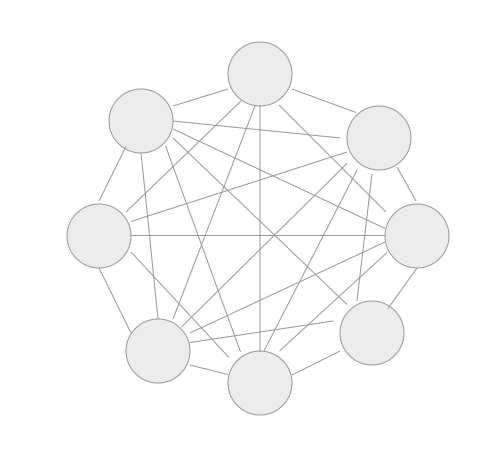
\includegraphics[scale=0.5]{img/many-to-many}
    \caption{Everyone makes channel with anyone else}
    \label{img:many-to-many}
\end{figure}

Many existing research on payment channels have focused on exploring the design
space of how to structure payments through intermediaries \cite{counterfactual, 
perun, lightning}. Let's suppose that Alice has a payment channel with Ingrid, and 
Ingrid has one with Bob. If Alice pays Ingrid off-chain and then Ingrid pays Bob 
the same amount, this is equivalent to Alice paying to Bob off-chain, without 
requiring a new Alice-Bob payment channel to be set up.

In situation when parties don't have channels with single intermediary, a 
micropayment channel network can be used together with a routing algorithm to 
send funds between any two parties in the network (see figure \ref{img:lightning}).

\begin{figure}[H]
    \centering
    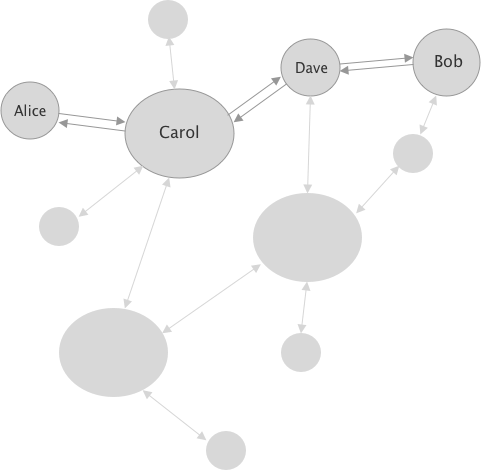
\includegraphics[scale=0.5]{img/lightning-network}
    \caption{Micropayment channels network}
    \label{img:lightning}
\end{figure}

As micropayment channel network can keep most transactions off-chain, blockchain 
based currencies may scale to magnitudes larger user and transaction volumes than 
any currently exsting centralised solution. Also, micropayment channel networks 
allow for fast transactions thanks to \textit{instant finality} property of 
payment channels. Transaction is final as soon as it is signed and sent to 
another party, the blockchain latency does not matter. \\

\subsubsection{Hashed Timelocked Contracts and Virtual Channels}

There are various ways to create micropayments networks trustlessly (i.e. to 
ensure that Alice pays Ingrid if Ingrid pays Bob). The most popular is Hashed 
Timelock Contract (HTLC) based approach \cite{lightning}. In it's canonical way 
an equal amount of funds from both payment channels are locked up in a way that 
they can only be spent if a certain hash is revealed before a certain deadline 
(thus, locked “by hash” and “by time”). 

This technique can allow payments to be securely routed across multiple payment 
channels and is used in Bitcoin's Lightning Network and Ethereum's Raiden 
Network.

\begin{figure}[H]
    \centering
    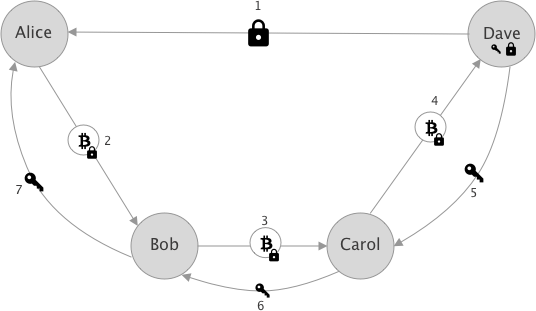
\includegraphics[scale=0.5]{img/htlc}
    \caption{HTLC based payment - Alice pays Dave}
    \label{img:htlc}
\end{figure}

In figure \ref{img:htlc} we see atomic value exchange over three micropayment 
channels (Alice to Bob, Bob to Carol, Carol to Dave). If Alice will pay to Dave
via Bob and Carol, she needs to ensure that Bob and Carol cannot run away with 
her money. To do so, Dave generates pre-image $R$, which is random number (shown 
as key on scheme), and then shared with Alice hash $H$ (shown as lock on scheme) 
of this pre-image. In step $2$ Alice generates an HTLC with Bob that says 
\textit{"I will pay you $X$ coins if you show me the pre-image $R$. If you don't 
show R during period $\Delta t$, I will take back my coins."}. In step $3$ Bob 
generates similar HTLC with Carol, but sets period of $\Delta t - 1$. In $4$ step 
Carol do same with Dave, but with even shorter period of $\Delta t - 2$. Then in 
step $5$ Dave will show $R$ to Carol, in next step Carol shows $R$ to Bob and 
finally Bob shows it to Alice. At this point payment of $X$ amount from Alice to 
Dave is finalsed.

HTLCs can be established in any chain of any length consisting of different 
payment channels. As an incentive for intermediate hops to forward transactionsa 
small fee can be charged for using the service of the channel. Fee payments are 
also justified as the balance on a channel gets shifted, which is only beneficial 
for balancing a lopsided channel. After a successful transaction with HTLCs, 
channel parties do not need to broadcast their contract and can just replace their
HTLC with a new commitment transaction without an HTLC. HTLCs can be combined with 
timelocks or revocable transactions changing the output of the HTLC accordingly.\\

In Ethereum blockchain, which supports advanced smart contracts, routing payments 
could be done in an alternative form via a technique known as \textit{Virtual 
channels}, introduced by \textit{Perun} paper \cite{perun} and simultaneously 
similar technique was proposed by \textit{Counterfactual} protocol (named as Meta 
channels), which use an intermediary that serves as a \textit{"virtual payments 
hub"}. Anyone with a payment channel connected to the hub could establish virtual
channels between each other (see figure \ref{img:hub}). Unlike routing payments 
via HTLCs, Hub does not need to be involved in every payment between Alice and 
Bob. This property reduces latency and costs, while increases privacy.

\begin{figure}[H]
    \centering
    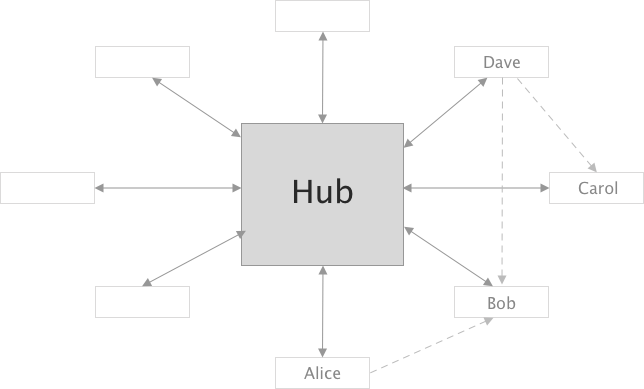
\includegraphics[scale=0.5]{img/hub}
    \caption{Virtual Payment Channel Hub}
    \label{img:hub}
\end{figure}

To open virtual channel, Alice and Bob essentially need to lock-up a set number
of coins from their payment channel with Hub. The amount of locked coins will 
become the value of the virtual channel between Alice and Bob. Notice, that the 
Hub remains financially neutral by simply mirroring balances.

This technique could be repplied to increase the length of the channel (see 
figure \ref{img:virtual-channels}). Because a virtual channel is an instance of 
an off-chain contract, increasing the length not require another transaction 
on-chain.

\begin{figure}[H]
    \centering
    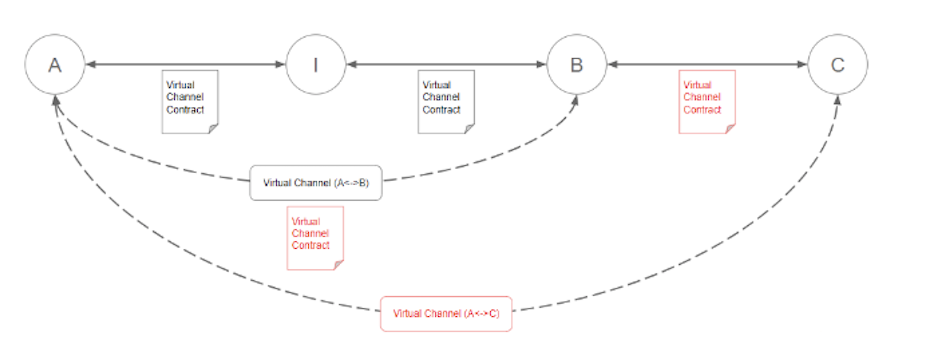
\includegraphics[scale=0.6]{img/virtual-channels}
    \caption{Bob becomes the Hub for channel between Alice and Carol}
    \label{img:virtual-channels}
\end{figure}

Virtual channels also represent a different business model from channel routing.
HTLCs have a \textit{“pay-per-payment”} fee model where there is need to 
incentivize each intermediary to route each payment. Virtual channels, on the 
other hand, have a \textit{“rent-a-path”} fee model. In this model, an 
intermediary acts as a virtual payment hub that has direct channels with multiple
parties. If Ingrid is the intermediary, then Alice and Bob pay Ingrid to keep 
the channel open for a certain period of time. Such a model might have better 
economics for high-volume micropayments.

While Perun and Counterfactual have introduced novel ways of routing payments 
across multiple intermediaries, HTLC-based routing is currently the primary 
implementation on blockchain mainnets, is better tested and much easier to 
implement.

\subsubsection{Known problems of micropayment networks}

Micropayment channels networks looks really promising but unfortunatelly they 
have couple of negative sides. 

Downside of using HTLC based micropayment networks is complicated routing. 
\textit{Lightning Network} is great for time to time low value payments, however 
it is much harder to use for frequent transactions into same receiver because of 
need of constantly checking if all parties in selected route are still alive and 
good to be used (e.g. all channels has enough funds to send payment forward).

Complicated routing issue could be solved by using payment hub model, when one 
of a fewnintermediaries have a lot of channels with end users. Downside of this 
solution is that this requires the Hub to lock a lot of funds in channels with 
all actors in the network. Another downside is that this solution is centralised 
and if hub's operator will be required to stop activities or will decide to 
shutdown servers by any reason, the whole network's payments activities will be 
stopped.

Another critique of payment channels network is that both parites (paying and 
receiving) have to be on-line during payment. This issue however is not valid for 
high frequency nano payments in decentralised networks, because we're sure, that
payer (service consumer) and payee (service provider) are on-line, otherwhise 
service wouldn't be provided and there would be no need for payment.

Finally, micropayment channel networks are really usefull when there are a lot
of people already using them. And when there are huge support for all popular 
programming languages and platforms. Unfortunatelly, them most popular solution
(Lightning Network) don't support tokens. On Ethereum there are a few promissing
projects (e.g. Raiden, Connext, Perun or Counterfactual), but they either are 
not widely adopted, either in early stage of development. Because they don't 
have rich tooling (e.g. protocol client implementations in popular languages 
like golang, rust or python) and are changing rapidly, they are quite 
complicated to implement and maintain. There are no clear winner at the moment
and trying to stick into one of general purpose payment network's could mean
choosing wrong direction which may mean either becoming main network developer,
either having complicated migration into another (much more popular at that 
time) solution in the future.

\subsection{Comparison and conclusion}

The key insight of \textit{Layer 2} soliutions is that not every transaction has
to be applied globally. All analysed solutions solves this problem in different 
ways and has different trade-offs. 

Many state channel developers see \textit{Layer 1} as the Security Layer and 
\textit{Layer 2} as the Scalability Layer. Furthermore, Layer 2 provides lower 
latency and cost per transaction that would otherwise not be possible beyond a 
certain level of throughput with Layer 1 solutions.

\begin{table}[H]\footnotesize
    \centering
    \caption{Comparison of researched solutions}
    {\begin{tabular}{|l|c|c|c|c|c|} \hline
       & \textbf{Channels} & \textbf{HTLC Network} & \textbf{Payment Hub} & \textbf{Plasma} & \textbf{Sidechain} \\
      \hline
      On-chain transactions & $\bullet\bullet\bullet$ & $\bullet\bullet$ & $\bullet\bullet$ & $\bullet$ & $\bullet$ \\
      Instant finality &  \checkmark &  \checkmark &  \checkmark & & \\
      Hight throughput & $\bullet\bullet$ & $\bullet\bullet\bullet$  & $\bullet\bullet\bullet$ & $\bullet$ & $\bullet$ \\
      Off-chain messaging & $\bullet$ & $\bullet\bullet\bullet$ & $\bullet\bullet$ & $\bullet$ & $\bullet$ \\
      Decentralised & \checkmark & \checkmark & $\pm$ & $?$ & $\pm$ \\
      Requires specialised wallet & $?$ & \checkmark & \checkmark & \checkmark & \checkmark \\
      Topup from exchange & $?$ & $-$ & $-$ & $-$ & \checkmark \\
      Easily embedable & \checkmark & $\pm$ & $-$ & $\pm$ & $\pm$ \\
      Overall user experience & $\bullet$ & $\bullet$ & $\bullet\bullet\bullet$ & $\bullet\bullet$ & $\bullet\bullet$ \\
      Implementation complexity & $\bullet$ & $\bullet\bullet\bullet$ & $\bullet\bullet$ & $\bullet\bullet\bullet$ & $\bullet\bullet\bullet$ \\
      Fast settlement & $?$ & $-$ & $\pm$ & \checkmark & $-$ \\
      Security & $\bullet\bullet\bullet$ & $\bullet\bullet\bullet$ & $\bullet\bullet\bullet$ & $\bullet\bullet\bullet$ & $?$ \\
      Utility token support & \checkmark & \checkmark & \checkmark & \checkmark & \checkmark \\
      \hline
    \end{tabular}}
    \label{tab:comparison}
  \end{table}

Explanation of meaning of used symbols: 
$\bullet\bullet\bullet$ -- high, 
$\bullet\bullet$ -- medium, 
$\bullet$ -- low, 
\checkmark -- yes, 
$\pm$ -- more or less, 
$?$ -- unknown, depends on implementation. \\

Explanation of compared solutions:

\begin{itemize}
    \item \textbf{Channels} -- pure payment channels bease solution (without 
    network), when each pair of consumer and provider have to open new channel.
    \item \textbf{HTLC Network} -- Micropayment channels networks which is using
    hashed timelocked contracts for payment routing, e.g. Raiden Networks.
    \item \textbf{Payment Hub} -- Virtual channels hubs based payment solution,
    such as Perun, Counterfactual or Connext.
    \item \textbf{Plasma} -- One of Plasma chain implementations (e.g. Plasma 
    MVP), dedicated to serve for payment purposes for particular distributed
    system.
    \item \textbf{Sidechain} -- Running sidechain using Substrate or Tendermint
    frameworks and connected to Polkadot or Cosmos.
\end{itemize}

In table \ref{tab:comparison} we can see comparison of properties given by 
analysed solutions. It is clear, that because of \textit{instant finality} and 
higher throughput posibilities, micropayment channels based solutions (such as
state channels, htlc networks or virtual payment hubs) fits better for high 
freakquency micropayments in decentralised platforms.

\section{Accountant pattern - lightweight payment protocol}

After analysing currently available options became obvious that at this stage
it may be better solution to introduce own, lightweight, state channels based,
easy to implement and maintain solution. 

In this section idea of \textit{"Accountant pattern"} protocol will be 
described. Essentially it is solution taking best parts of Payment promises,
uni-directional channles and paying using single intermediary taking use of 
hashed timelocked contracts for avoding need of introducing trusted custodian.

\subsection{Payments over "Accountant"}

Digital cheques or \textit{Payment promises} is elegant, efficient and easy to 
implement solution. Thanks to some modifications (comparing to initial solution,
described in 2.2 section) they have to be signed by only one party, are easy to 
verify, don't require complicated setup procedure, have practically unlimited 
amount of updates and require to store only last version of issued promise.

Main problems of using them is possibility to do double spending which pushes 
for more often on-chain settlements. To solve this problem there is suggestion 
to introduce one more party called \textit{Accountant} which should see and 
verify promises issued by consumer and be aware of actual balance of consumer's
funds (see figure \ref{img:unidirectional-payments}).

\begin{figure}[H]
    \centering
    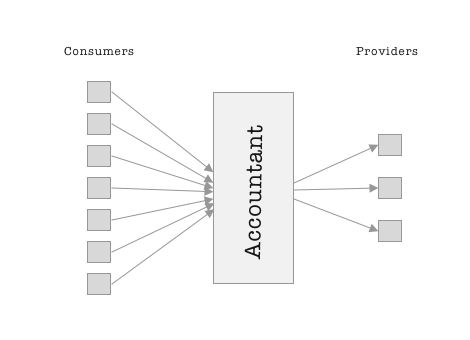
\includegraphics[scale=0.5]{img/unidirectional-payments}
    \caption{Payments via Accountant}
    \label{img:unidirectional-payments}
\end{figure}

Accountant is the most complicated to implement part of this protocol. He have 
to store state of balance of each consumer and be able to accept many requests 
to validate if transaction is valid.

\begin{figure}[H]
    \centering
    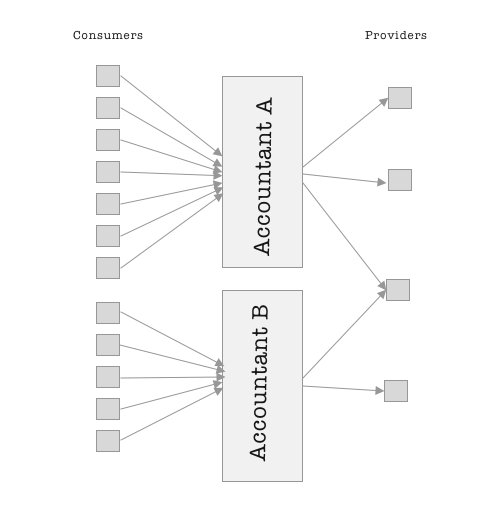
\includegraphics[scale=0.5]{img/multi-accountants}
    \caption{Multiple accountants may be used in network}
    \label{img:multi-accountants}
\end{figure}

To maintain requirement of decentralisation there may be deployed multiple 
accountants in the network (see figure \ref{img:multi-accountants}). Each 
consumer usually works with only one accountant while providers may need to be 
aware of different accountants. Accountants are chosen by consumers but because 
of cryptographic schemes described in next sections they are non-custodian and 
can't steal any funds or cooperate with consumers to cheat against providers.

\subsection{Payment Promises based uni-directional channels}

To organise secure, non-custodian and trustless work via accountant, we have to 
maintain two types of channels: paying channels (consumer $\rightarrow$ 
accountant) and receiving channels (accountant $\rightarrow$ provider). So 
accountant plays similar role as intermediary or hub described in section 3.3.3.

\begin{figure}[H]
    \centering
    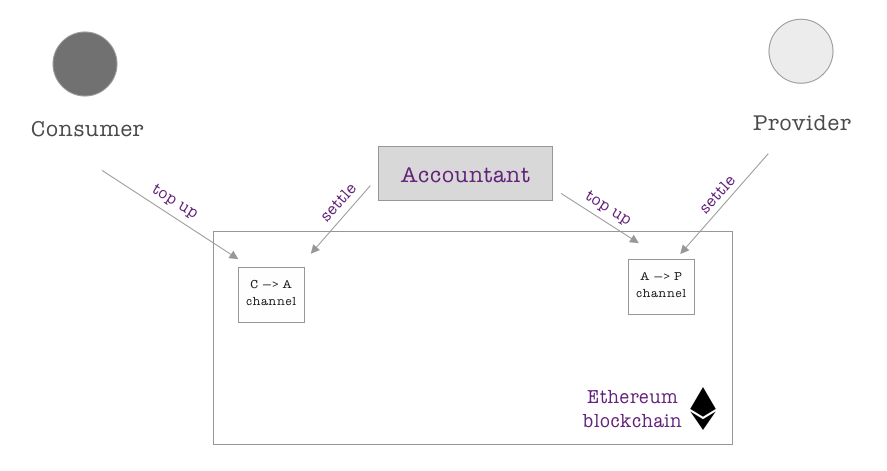
\includegraphics[scale=0.4]{img/accountant-channels}
    \caption{Two type of channels}
    \label{img:accountant-channels}
\end{figure}

Because in our case we have situation when payments are done in one direction 
(from consumer to provider) we may organise uni-directional state channels 
which are very similar to payment promises and have most of their properties. 
The only differences are that there should be done accounting and funds freezing 
for each channel separately. Also hashlock check (HTLC described in section 
3.3.4) was added to guaranty that Accountant will not keep funds to itself.

Implementation of promise settlement function can be found above and full 
state channel smart contract can be found in github repository 
\cite{smartcontracts}.

\begin{lstlisting}[language=Solidity]
    struct Party {
        address beneficiary; // funds destination
        uint256 settled;     // total amount already settled
    }

    function settlePromise(uint256 _amount, bytes32 _lock, bytes memory _signature) public {

        bytes32 _hashlock = keccak256(abi.encode(_lock));
        address _channelId = address(this);

        address _signer = keccak256(abi.encodePacked(
                _channelId, 
                _amount, 
                _hashlock
        )).recover(_signature);
        require(_signer == operator);

        // Calculate amount of tokens to be settled.
        uint256 _unpaidAmount = _amount.sub(party.settled);
        require(_unpaidAmount > 0);

        // If signer has less tokens than asked to transfer, 
        // we can transfer as much as he has already and rest 
        // tokens can be transferred via same promise but in 
        // another tx when signer will topup channel balance.
        uint _currentBalance = token.balanceOf(_channelId);
        if (_unpaidAmount > _currentBalance) {
            _unpaidAmount = _currentBalance;
        }

        // Increase already paid amount
        party.settled = party.settled.add(_unpaidAmount);

        // Send tokens
        token.transfer(party.beneficiary, _unpaidAmount);
    }
\end{lstlisting}

Because our channels are uni-directional instead of sequence number there is 
simply used total promised amount. Smart contract is calculating difference 
between amount on given promise and already settled amount.

\[ amountToTransfer = totalPromised - alreadySettled \]

This gives high level of flexibility. Promises can be settled in any order with
any gaps (e.g. only one of thousand promised can be send to settle) and amounts 
still will be calculated properly.

\subsection{Identity registry}

Another important component of protocol is \textit{registry} where all 
identities (both, consumers and providers) and accountants should be registered. 
During registration there will be also created payment channel between consumer 
and accountnat (see figure \ref{img:registration}).

\begin{figure}[H]
    \centering
    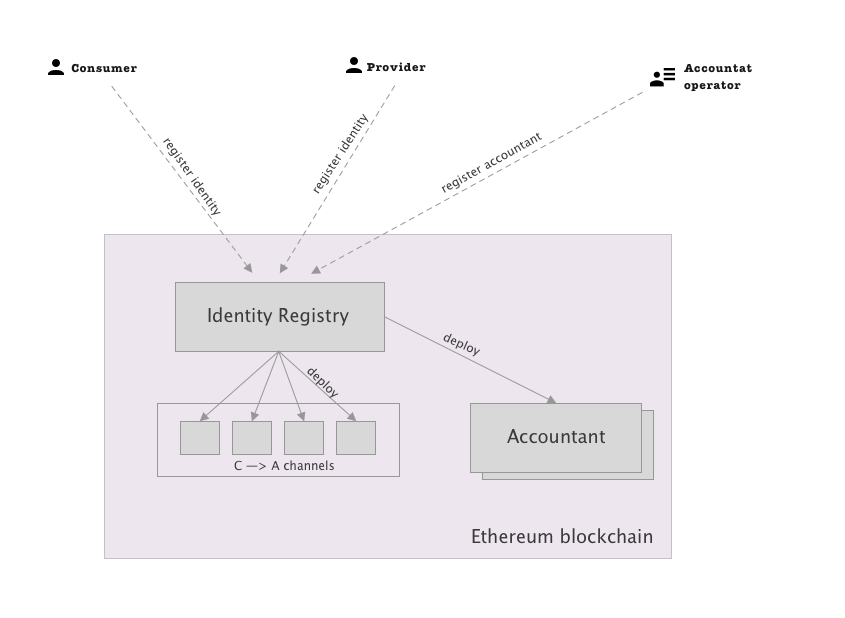
\includegraphics[scale=0.4]{img/registration}
    \caption{Registration of accountant and identities}
    \label{img:registration}
\end{figure}

Because there will be need to deploy channel per each registered identity there 
have to be done optimisation in terms to save of channel deployment transaction 
fee. This protocol suggests to use \textit{EIP1167} (Minimal Proxy Contract 
\cite{eip1167}) which will proxy all requests into single 
\textit{ChannelImplementation} contract while still allow to maintain separate 
state and address per each channel (see figure \ref{img:proxy}).

\begin{figure}[H]
    \centering
    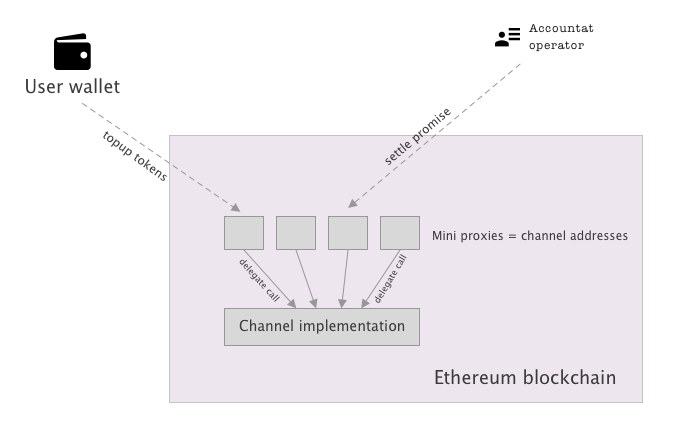
\includegraphics[scale=0.5]{img/proxy}
    \caption{Minical proxies pointing into single implementation}
    \label{img:proxy}
\end{figure}

Consumer (paying) channels are deployed using \textit{CREATE2} opcode \cite{create2} 
which allows deterministically calculate future channel's address.

\[ keccak256(0xff + registry + identity + keccak256(byteCode))[12:]\]

This means, that users can topup their channels even before identity was 
registered and actual smart contract code was deployed there. Also because each
channel has separate address and it's topup don't require adding any aditional 
parameters (payload) to the transaction, they can be topuped using any wallet 
with token support or directly from exchange.

\subsection{Off-chain messaging and promise exchange}

Differently than in \textit{Lightning Network} or \textit{Hub} based payment 
networks, in \textit{Accountant pattern} payments are not going thgrough 
intermediary, but are "verified" by Accountant. There is used payment promise 
exchange technique (see figure \ref{img:off-chain-interactions}).

\begin{figure}[H]
    \centering
    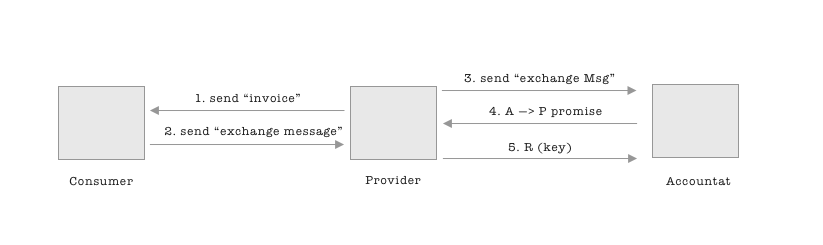
\includegraphics[scale=0.5]{img/off-chain-interactions}
    \caption{HTLC based payment - Bob pays Alice}
    \label{img:off-chain-interactions}
\end{figure}

Payment is finalised in five steps. At fist Provider have to \textit{generate 
invoice} and send it to Consumer.

\[ invoice = [hashlock, agreementId, agreementAmout] \]
\[ hashlock = keccak256(R) \]
\[ R = HugeRandomNumber \]

Then Consumer issues payment promise, which allows Accountant to settle given 
amount of funds, pack it into so called \textit{Exchange message} and send back 
to Provider. 

\[ Message = keccak256(channelId, totalPromisedAmount, hashlock) \]
\[ Signature = sign(Message) \]
\[ Promise = [Message, Signature]\]
\[ ExchangeMessage = [Promise, agreementId, agreementAmout] \]

In next steps Provider is exchanging promises with Accountant so in the end 
Accountant have promise to settle funds in Consumer's channel and Provider 
have payment promise to settle same amount of funds in Accountant's channel.

\[ \Delta amount = newAgreementAmout - seenAgreementAmout \]
\[ totalPromisedAmount = previousPromisedAmount + \Delta amount \]

Provider can do same promise exchange operations with many consumers at once. 
After any number of succesfull off-chain interactions, provider at any point, 
in single transaction, can settle last payment promise with accomulated amount 
of payments done by couple of consumers (see figure \ref{img:payment}. 
Aditionally, if Provider is willing to take some risk (up to some amount) he 
can verify (exchange promises with accountant) not each payment and reduce 
amount of off-chain communication and fee paid to Accountant.

\begin{figure}[H]
    \centering
    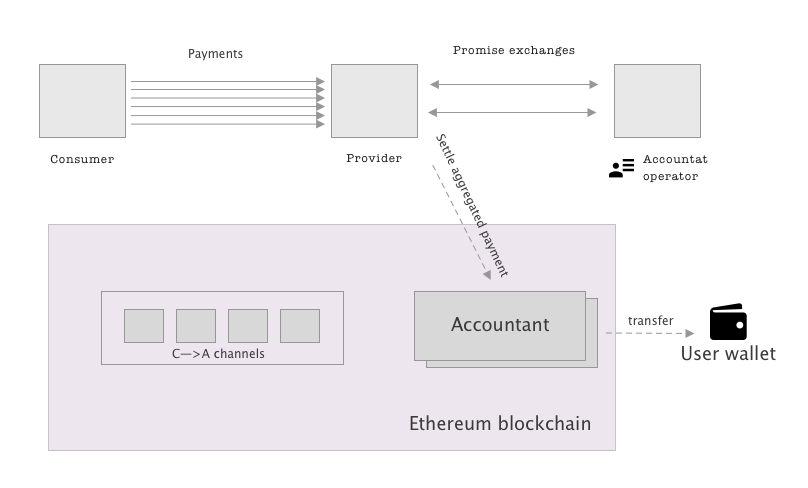
\includegraphics[scale=0.4]{img/payment}
    \caption{Provider settles aggregated promise}
    \label{img:payment}
\end{figure}

Accountant is also accomulating payment promises given by same Consumer to 
different Providers. When he will have payment promise with enought big value 
he can settle it on-chain (see figure \ref{img:accountant-rebalance}) and 
rebalance paying and receiving channels.

\begin{figure}[H]
    \centering
    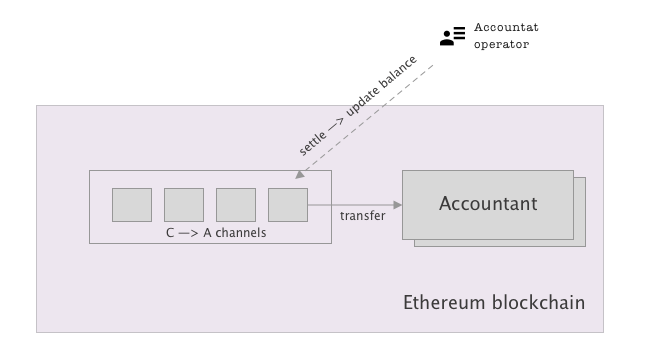
\includegraphics[scale=0.5]{img/accountant-rebalance}
    \caption{Accountant rebalancing is simple settlement of collected promises}
    \label{img:accountant-rebalance}
\end{figure}

\subsection{Incoming channel funds guaranties and trustless rebalance}

All analysed micropayment channel based solutions have common problem of need 
to lock funds in channels with each party. In hub based solutions this problem 
is even bigger and requires so called \textit{"rich hub"}. Thanks to possibiltiy 
to take stake and users separation to consumers and providers it is possible to 
decrease this problem.

\begin{lstlisting}[language=Vyper]
    lockedFunds: uint256 # amount of accountant funds already locked in channels
    struct Channel:
      loan: uint256      # amount lended by provider
      balance: uint256   # amount available to settle
      settled: uint256   # total amount settled by provider

    @public
    def rebalanceChannel(channelId: bytes32):
      newBalance: uint256 = channels[channelId].loan
      assert newBalance > channels[channelId].balance

      channel: Channel = channels[channelId]

      if(newBalance > channel.balance):
        lockedFunds += channel.balance - newBalance
        assert token.balanceOf(this) >= lockedFunds

      channel.balance = newBalance
\end{lstlisting}

Provider's stake can be taken and lended into Accounant and imidiatelly locked 
in his receiving payment channel. In this way, accountant will lock his own 
funds, which means that Provider can settle payment promises in value of up to 
his stake size.

Additional benefit is that Accountant can't actually withdraw and use these 
funds, so channel rebalance can be done by anyone, without accountant's 
signature.

"Always online" is big problem for payment channels. If Provider is offline or 
is under DDoS attack, he will be unable to post the finalized state (during 
dispute period) and Accountant can have possibility to take funds locked in 
channel.

Proposed method don't have such problem, because funds are double locked. 
Accountant can't leave channel with more funds than his own locked part of 
balance. So if Provider have unsettled promise for smaller amount than he 
lended to Accountant, he is safe even if he will "dissapear" for really long 
period of time. He still be able to get back all funds promised to him.

\subsection{Transaction maker and watch towers}

One of most not user friendly parts of transfering ERC20 tokens is that this
operation requires to also own ethers to pay for gas. Another problem in
working with smart contracts on Ethereum is that in terms to call some function
user have to add so called Payload (first 4 bytes of keccak of function's
signature) which looks to his as abracadabra and is not supported by many 
wallets and especially by exchanges. 

In case of topups, this problem is solved thanks to construct described in 4.3
section. Unfortunatelly for identity registration and promise settlement, user's 
application (e.g. dVPN mobile app or provider's node) would need to always have 
ethers topuped there. This is very inconvenient and may cause many problems for
both advanced users and beginners.

\begin{figure}[H]
    \centering
    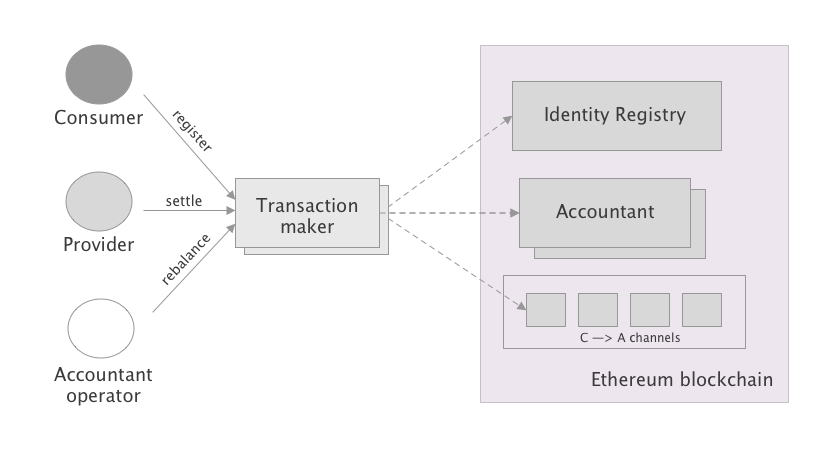
\includegraphics[scale=0.5]{img/transactor}
    \caption{Communication with blockchain via Transaction maker}
    \label{img:transactor}
\end{figure}

For identity registration and primise settlement we may take use of additional
service which we call \textit{"Transaction maker"}. The role of this service is 
to get user's requests and send transactions into blockchain (see figure 
\ref{img:transactor}).

All smart contracts created for Accounant pattern are constructed in a way, so
any their call can be made from any account simply by adding channel's operator
signature ar parameter into payload. Additionaly we construct payment promises 
in a way so only one signature is needed and it is possibile to settle them in 
any order with any gaps. This means that promises can we publicated publicly
without any risk of attack.

There could be deployed as many such services as needed.
Each network participant could decide to use own \textit{"Transaction maker"},
or even there could be version of accountant operator software where such 
service is integral part.

Sending transactions into blockchain costs so users could cover that cost, but
instead of using additional currency (ethers in case of Ethereum), they could
pay in tokens, and as payment mechanism Payment promises (described in sections
4.2 and 4.4) could be used (see figure)

\begin{figure}[H]
    \centering
    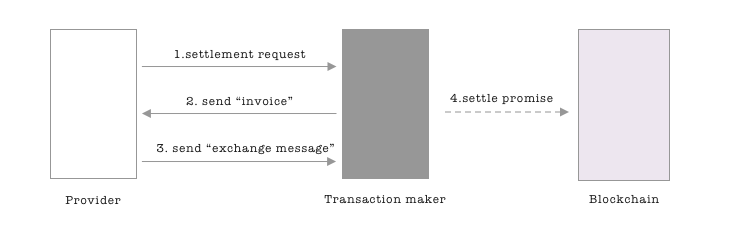
\includegraphics[scale=0.5]{img/transactor-payment}
    \caption{Paying via Tramsaction maker flow}
    \label{img:transactor-payment}
\end{figure}

\subsection{Properties of the protocol}

This protocol was design to be integral part of some decentralised system and 
is not aimed to work as general purpose payment network used in many 
application and daily life, when each party in the same time can receive and 
send funds. 

Main properties of protocol are:

\begin{itemize}
  \item Easy paying channel topup (even from exchange).
  \item Payments aggregation $\Longrightarrow$ minimal on-chain tx amount.
  \item Fast settlement into blockchain without need for other party to be on-line
  and cooperate.
  \item Guaranty of incomming channel balance/collateral size.
  \item Simple off-chain communication (one roundtrip payments).
  \item Possibility to avoid accountant for at least part of transactions.
  \item Pull based interations with accountant $\Longrightarrow$ providers don't have to
  be externally exposed or maintain live connection with accountant.
  \item Secure $\Longrightarrow$ double spend protection using non-custodian accountant
  model.
  \item Fast channel opening $\Longrightarrow$ possibility not to wait until opening tx
   will be mined.
  \item Instant finality of payments.
\end{itemize}

\subsection{Potential future work}

- Migrate into Connext or Perun 
- Migrate into Plasma + channels
- Accountant support Counterfactual channels


Author has plans to research possibility to apply similar model for UTXO based statefull 
chains, such as Cardano or Plasma MVP. Also there is willing to research what would be 
possible to do on Bitcoin blockchain or how to create lightweight hub for Lightning 
Network.

Identity channels could be implemented as multisig contracts done in 
\textit{Counterfactual} \cite{counterfactual} way, so in the future there would be 
possible introduce new payment channels types without need of creating new channels of 
doing any other on-chain action or upgrade of deployed smart-contracts. 

In the future there may be discovered potential applicability of \textit{channel 
factories} \cite{factories} as way for cross hub communication which may reduce need 
for users to establish connections with many hubs. This potentially increase 
decentralisation of the network while maintaining same scalability properties (avoiding 
complex routing used in Lightning Network).


\newpage
\printbibliography[heading=bibintoc]

\end{document}
